\noindent Throughout this document we use the word \textbf{limb}\label{def: limb} to designate a $\llarge$-byte integer.

% \ob{TODO: representation of RAM with \cnA{}, \indexA{}, \valA{}, $\valA{}\new{}$ etc \dots{}}
The RAM data processor has, at all times, access to precisely 3 values (limbs) from RAM. These values can be chosen from distinct execution contexts, including the $0^{\text{th}}$ execution context which plays a special role. To specify a ``value in RAM'' we thus require a tuples consisting of (a) an execution context (b) a limb offset in RAM (c) the limb (i.e. value) stored at that offset. The arithmetization requires us to add to these (d) a \emph{potentially} udpated value of that limb and (e) bytes that \emph{potentially} spell out the byte decomposition of the limb currently in RAM (i.e. before any \emph{potential} update). This is the purpose of the following columns. Since the RAM data processor can access three RAM slots there are three such quintuples. We give more details below.

Three \emph{counter-constant columns} containing execution context numbers:
\begin{enumerate}
	\item \CNA{}; abbreviated to \cnA{};
	\item \CNB{}; abbreviated to \cnB{};
	\item \CNC{}; abbreviated to \cnC{};
\end{enumerate}
Three \emph{counter-constant columns} containing limb offsets within the corresponding execution context's RAM:
\begin{enumerate}[resume]
	\item \indexA{}: limb offset in the RAM of context \cnA{};
	\item \indexB{}: limb offset in the RAM of context \cnB{};
	\item \indexC{}: limb offset in the RAM of context \cnC{};
\end{enumerate}
Three \emph{counter-constant columns} containing the limbs currently stored at the given offsets inside the corresponding execution context's RAM:
\begin{enumerate}[resume]
	\item \VALA{}: (limb) value currently in \cnA{}'s RAM at \indexA{}; abbreviated to \valA{};
	\item \VALB{}: (limb) value currently in \cnB{}'s RAM at \indexB{}; abbreviated to \valB{};
	\item \VALC{}: (limb) value currently in \cnC{}'s RAM at \indexC{}; abbreviated to \valC{};
\end{enumerate}
Three \emph{counter-constant columns} containing \emph{potentially} updated values of the limbs currently stored at the given offsets inside the corresponding execution context's RAM:
\begin{enumerate}[resume]
	\item \VALANEW{}; updated value in \cnA{}'s RAM at \indexA{}; abbreviated to $\valA{}\new$;
	\item \VALBNEW{}; updated value in \cnB{}'s RAM at \indexB{}; abbreviated to $\valB{}\new$;
	\item \VALCNEW{}; updated value in \cnC{}'s RAM at \indexC{}; abbreviated to $\valC{}\new$;
\end{enumerate}
Three \emph{byte columns} which \emph{may} contain the byte decompositions of \valA{}, \valB{} and/or \valC{} (depending on whether they are required for the present computation):
\begin{enumerate}[resume]
	\item \BYTEA{}; byte columns; % abbreviated to \byteA{};
	\item \BYTEB{}; byte columns; % abbreviated to \byteB{};
	\item \BYTEC{}; byte columns; % abbreviated to \byteC{};
\end{enumerate}
We also require three \emph{accumulator columns} which \emph{may} witness these byte decompositions:
\begin{enumerate}[resume]
	\item \acc{A}: if $\slowOp{} = 1$ accumulates the bytes of the \byteA{} column;
	\item \acc{B}: if $\slowOp{} = 1$ accumulates the bytes of the \byteB{} column;
	\item \acc{C}: if $\slowOp{} = 1$ accumulates the bytes of the \byteC{} column;
\end{enumerate}
\begin{figure}
\centering
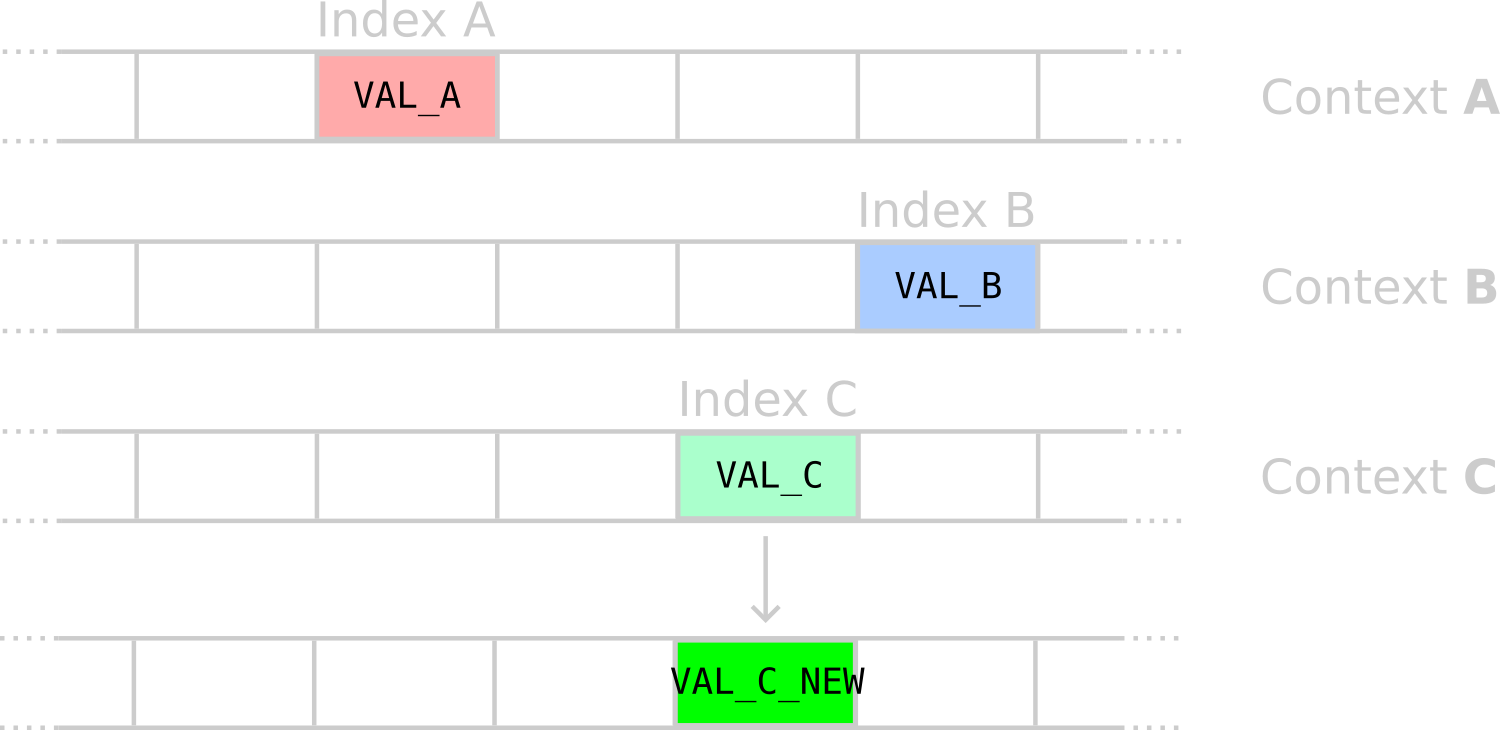
\includegraphics[width = 0.7\textwidth]{drawing/bla}
\caption{The diagram above contains all the intuition there is to convey about context numbers, indices, values and updated values. Every execution context (identified by its context number) has its own RAM, the data in RAM is addressed via an index $\in\{0,1,\dots\}$ which for the purposes of the zk-evm always is a $\ssmall{}$-byte integer as larger offsets are rejected before getting this far. The data itself is packaged as ``limbs'': $\llarge{}$-byte integers. Instructions may change 0, 1, 2 or even three of the available RAM limbs at any point in time. In the above only the $\VALC$ is modified.}
\end{figure}

The RAM pre-processor converts RAM instructions into a sequence of \textbf{RAM micro instructions}\label{def: RAM micro instruction}. The RAM data processor only knows how to deal with micro instructions. Micro instructions can be fast ($\fastOp = 1$) or slow ($\fastOp = 0$). Fast micro instructions take up exactly one row in the RAM data processor's execution trace. Slow micro instructions take up exactly $\llarge$ rows in the RAM data processor's execution trace. RAM micro instructions can modify 1, 2 or even 3 limbs at once through various forms of \textbf{limb surgery}. These limbs may be in RAM, imported from the stack or part of exogenous data. The modification can use as inputs 1, 2 or even 3 limbs taken from RAM, the stack or exogenous data. Limb surgeries (micro instructions that modify limbs on a byte level) are determined by their \emph{(data) source}, \emph{(data) target}, a \emph{surgery pattern} and an \emph{offset} and potentially a \emph{size}. The micro instruction, the source and target, the offsets and the size (if any) are handed down to the RAM data processor from the pre-processor. Offsets are actually given in terms of a \emph{limb offset} and a \emph{byte offset} determined by euclidean division of the underlying offset by 16: 
\[
	\textsf{offset} = 16\cdot \textsf{limbOffset} + \textsf{byteOffset},
	\quad
	\textsf{byteOffset} \in \{0,1,\dots,\llargeMO\}.
\]

The following are columns \textbf{imported} from the RAM preprocessor. Colums that are imported from the RAM preprocessor are distinguished by angular brackets as in $\imported{\col{X}}$. \emph{All imported columms are counter-constant}.
\begin{enumerate}[resume]
	\item $\mmioStamp{}$: contains the \mmioMod{} stamp;
	\item $\mmioInst{}$: contains the \mmioMod{} instruction of the current $\mmioStamp{}$;
	\item $\CNS{}$: context number of the context whose RAM \emph{may} be used as a source of limbs; abbreviated to $\cnS{}$;
	\item $\CNT{}$: context number of the context whose RAM \emph{may} be used as a target of limbs; abbreviated to $\cnT{}$;
	\item $\SLO{}$: this imported column contains the limb offset of the first limb to read from / write to in $\cnS{}$'s RAM; abbreviated to $\slo{}$
	\item $\TLO{}$: this imported column contains the limb offset of the first limb to read from / write to in $\cnT{}$'s RAM; abbreviated to $\tlo{}$
	\item $\SBO{}$: this imported column contains the byte offset within the limb to read from / write to in $\cnS{}$'s RAM; with values in $\{0,1,\dots, \llargeMO\}$; abbreviated to $\sbo{}$;
	\item $\TBO{}$: this imported column contains the byte offset within the limb to read from / write to in $\cnT{}$'s RAM; with values in $\{0,1,\dots, \llargeMO\}$; abbreviated to $\tbo{}$;
	\item $\size{}$: an imported column containing a ``size'' parameter used by certain limb surgeries;
	\item $\limb{}$: an imported column containing a ``limb'';
	\item $\totalSize{}$: an imported column containing the total size of the output of the $\mmuInstAnyToRamWithPadding$;
	\item $\exoSum{}$: an imported column containing an integer that is understood as a bit field; is decoded into flags to impose in which exo module read or write the limbs;
	\item $\idOne{}$ and $\idTwo{}$: contain an identifier (stamp) of the needed exo module;
	\item $\Phase{}$: contains the ``phase'' in the exo module to specify, for a given ``stamp'' at which rows the lookup occurs;
	\item $\successBit{}$: bit column; contains the success (or failure) of the current evm operation;
		% TODO: add new macros and replace them everywhere in the MMIO module spec
		% µ/XX MMIO/XX 
		% \item $\mmioStamp{}$: contains the \mmioMod{} stamp;
		% \item $\mmioInst{}$: contains the \mmioMod{} instruction of the current $\mmioStamp{}$;
		% \item $\CNS{}$: context number of the context whose RAM \emph{may} be used as a source of limbs; abbreviated to $\mmioCnS{}$;
		% \item $\CNT{}$: context number of the context whose RAM \emph{may} be used as a target of limbs; abbreviated to $\mmioCnT{}$;
		% \item $\SLO{}$: this column contains the limb offset of the first limb to read from / write to in $\mmioCnS{}$'s RAM; abbreviated to $\mmioSlo{}$
		% \item $\TLO{}$: this column contains the limb offset of the first limb to read from / write to in $\mmioCnT{}$'s RAM; abbreviated to $\mmioTlo{}$
		% \item $\SBO{}$: this column contains the byte offset within the limb to read from / write to in $\mmioCnS{}$'s RAM; with values in $\{0,1,\dots, \llargeMO\}$; abbreviated to $\mmioSbo{}$;
		% \item $\TBO{}$: this column contains the byte offset within the limb to read from / write to in $\mmioCnT{}$'s RAM; with values in $\{0,1,\dots, \llargeMO\}$; abbreviated to $\mmioTbo{}$;
		% \item $\mmioSize{}$: a column containing a ``size'' parameter used by certain limb surgeries;
		% \item $\mmioLimb{}$: a column containing a ``limb'';
		% \item $\mmioTotalSize{}$: a column containing the total size of the output of the $\mmuInstAnyToRamWithPadding$;
		% \item $\mmioExoSum{}$: a column containing an integer that is understood as a bit field; is decoded into flags to impose in which exo module read or write the limbs;
		% \item $\mmioIdOne{}$ and $\idTwo{}$: contain an identifier (stamp) of the needed exo module;
		% \item $\mmioPhase{}$: contains the ``phase'' in the exo module to specify, for a given ``stamp'' at which rows the lookup occurs;
		% \item $\mmioSuccessBit{}$: bit column; contains the success (or failure) of the current evm operation;
\end{enumerate}

The following are binary columns \textbf{decoded} from the previous \textbf{imported} columns: 
\begin{enumerate}[resume]
	\item \isMmioInstLimbVanishes{}                           
	\item \isMmioInstLimbToRamTransplant{}     
	\item \isMmioInstLimbToRamOneTarget{}
	\item \isMmioInstLimbToRamTwoTarget{}          
	\item \isMmioInstRamToLimbTransplant{} 
	\item \isMmioInstRamToLimbOneSource{}
	\item \isMmioInstRamToLimbTwoSource{}
	\item \isMmioInstRamToRamTransplant{}     
	\item \isMmioInstRamToRamPartial{}
	\item \isMmioInstRamToRamTwoTarget{}
	\item \isMmioInstRamToRamTwoSource{}
	\item \isMmioInstRamExcision{}                
	\item \isMmioInstRamVanishes{}            
	\item \fastOp{} and \slowOp{}: binary flag, indicates whether a micro instruction is fast (i.e. occupies a single line in the RAM data processor) or slow (i.e. occupies 16 consecutive lines in the RAM data processor.)
	\item \isExoFlagRom         {}
	\item \isExoFlagKec         {}
	\item \isExoFlagLog         {}
	\item \isExoFlagRlpTxn      {}
	\item \isExoFlagEcdata      {}
	\item \isExoFlagRipSha      {}
	\item \isExoFlagBlakeModexp {}
	\item \indexX{}: contains the limb offset of exogenous data;
	\item \byteLimb{}: byte column; \emph{may} contain the byte decomposition of $\limb{}$;
	\item \acc{LIMB}: if $\slowOp{} = 1$ accumulates the bytes of the \byteLimb{} column;
\end{enumerate}
We now introduce some columns that are of use in producing proofs but aren't meaningful outside of that.
\begin{enumerate}[resume]
 	\item ``binary plateau'' columns $\bit{1}, \bit{2}, \bit{3}, \bit{4}, \bit{5}$;
 	\item ``accumulator'' columns \acc{1}, \acc{2}, \acc{3}, \acc{4};
 	\item ``powers of 256'' columns $\pow{1}$ and $\pow{2}$;
 	\item \CT{}: a column that either hovers around 0 or counts up from 0 to $\llargeMO$ and resets to 0; used for slow memory operations (i.e. when $\slowOp{}=1$) when byte decompositions are needed;
\end{enumerate}
